\documentclass[twocolumn,10pt]{confpaper}
\usepackage{usenix,epsfig,url,amssymb,CJKutf8}
\usepackage{balance}
\usepackage{titling}
\begin{document}


%make title bold and 14 pt font (Latex default is non-bold, 16 pt)

\title{\fontsize{14}{14} \textbf{Automatically Generating a Large, \\ Culture-Specific Blocklist for China}}
\date{}
%for single author (just remove % characters)
\author{
{\rm Austin Hounsel}\\
Princeton University
\and
{\rm Prateek Mittal}\\
Princeton University
\and
{\rm Nick Feamster}\\
Princeton University
% copy the following lines to add more authors
% \and
% {\rm Name}\\
%Name Institution
} % End author

\posttitle{\par\end{center}}
\setlength{\droptitle}{-10pt}
\maketitle

% Use the following at camera-ready time to suppress page numbers.
% Comment it out when you first submit the paper for review.
\thispagestyle{empty}



\begin{abstract}
Internet censorship measurements rely on lists of websites to be
tested, or ``block lists'' that are curated by third parties.
Unfortunately, many of these lists are not public, and those that are
tend to focus on a small group of topics, leaving other types of sites
and services untested. To increase and diversify the set of sites on
existing block lists, we use natural language processing and search
engines to automatically discover a much wider range of websites that
are censored in China. Using these techniques, we create a list of 1125
websites outside the Alexa Top 1,000 that cover Chinese politics,
minority human rights organizations, oppressed
religions, and more. Importantly, \textit{none of the sites we discover are
present on the current largest block list}. The list that we develop
not only vastly expands the set of sites that current Internet
measurement tools can test, but it also deepens our understanding of
the nature of content that is censored in China. We have released both
this new block list and the code for generating it.
\end{abstract}

\section{Introduction} 

Internet censorship is pervasive in China. Topics ranging from
political dissent and religious assembly to privacy-enhancing
technologies are known to be
censored~\cite{citizenlab:block}. However, the Chinese government has
not released a complete list of websites that they have
filtered.~\cite{fhouse:china}. When performing measurements of
Internet filtering, then, the inability to know what sites are blocked
creates a circular problem of discovering the sites to measure in the
first place. To do so, various third parties currently curate lists of
websites that are known to be censored, or ``block lists''. These
lists are used to both understand {what} content is censored in China
and how that censorship is implemented. Indeed, the Open Observatory
of Network Interference notes that ``censorship findings are only as
interesting as the sites and services that you
test.''~\cite{ooni:lists}.

Instead of curating a block list by hand, Darer et al. proposed a
system called FilteredWeb that automatically discovers web pages that
are censored in China~\cite{darer2017filteredweb}. Their approach is
summarized in the following steps. First, keywords are extracted from
web pages on the Citizen Lab block list, a small, hand-curated
list. These are English words that are ranked through TF-IDF, a
technique which we describe in Section ~\ref{tf-idf}. Then, each
keyword is used as a query for a search engine, such as Bing. The
intuition is that censored web pages contain similar keywords. Finally,
each web page that appears in the search results is tested for DNS
manipulation in China. These tests are performed by sending DNS
queries to IP addresses in China that don't belong to DNS servers. If
a DNS response is received, then, it is inferred that the request was
intercepted in China and that the website is censored. Each
web page that is censored is fed back to the beginning of the
system. FilteredWeb discovered 1,355 censored domains, 759 of which
are outside the Alexa Top 1,000.

In this paper, we build upon the approach of FilteredWeb in the
following ways. First, {\em we extract content-rich phrases
for search queries}. In contrast, FilteredWeb only uses single words
for search queries. These phrases provide greater context regarding
the subject of censored web pages, which enables us to find websites
that are very closely related to each other. For example, consider the
phrase \begin{CJK*}{UTF8}{gbsn}中国侵犯人权 \end{CJK*} (Chinese human
rights violation). When we perform the searches \texttt{Chinese},
\texttt{human}, \texttt{rights} , and \texttt{violation}
independently, we mainly get websites for Western media outlets, many
of which are known to be censored in China. By contrast, if we search
for \texttt{Chinese human rights violation} as a single phrase, then
we discover a significant number of websites related to Chinese
culture, such as homepages for activist groups in China and
Taiwan. Identifying and extracting such key phrases is a non-trivial
task, as we discuss later.

Second, we use natural language processing to parse Chinese text
when adding to the blocklist. In contrast, FilteredWeb only extracts English
words that appear on a web page. As such, \textit{any website that is written
in simplified Chinese is ignored}, neglecting a significant portion of
censored sites. For example, there are many censored websites and blogs that
cover Chinese news and culture, and many of them only contain Chinese text. As
such, to discover region-specific, censored websites, such a system should be
able to parse Chinese text. Because Chinese is typically written without
spaces separating words, this requires the use of natural-language processing
tools.

Third, we make our block list public, in contrast to previous work. The
authors of FilteredWeb made their block list available to us for validation;
we have published our block list so others can build on
it~\cite{censorsearch-lists}.

In summary, we built and now maintain a large, public, culture-specific list
of websites that are censored in China. These websites cover topics such as
political dissent, historical events pertaining to the Chinese Communist
Party, Tibetan rights, religious freedom, and more. Furthermore, because many
of these website are written from the perspective of Chinese nationals and expatriates,
we are able to get first-hand accounts of Chinese culture that are
not present in other block lists. This new resource can help researchers who
are interested in studying Chinese censorship from the perspective of
marginalized groups that most affected by it.

In this paper, we make the following contributions:
\begin{itemize}
  \item We build upon the approach of FilteredWeb to discover censored
websites in China that specifically pertain to its culture. We do so
by extracting potentially sensitive Chinese phrases from censored
web pages and using them as search terms to find related websites.
  \item We build a list of 1125 censored domains in China, which is
12.5$\times$ larger than the standard list for censorship
measurements~\cite{citizenlab:block}. Furthermore, \textit{none of
these websites are on the largest block list
available}~\cite{darer2017filteredweb}.
  \item We perform a qualitative analysis of our block list to
    showcase its advantages over previous work.
\end{itemize}

The rest of the paper proceeds as follows. First, we describe our
approach to building a large, culture-specific block list for
China. This includes an in-depth analysis of the advantages of our
approach over previous work. Then, we describe three large-scale
evaluations that we performed. Each of these evaluations
produced qualitatively different results due to different
configurations of our system. Finally, we conclude
with a discussion of how the block list we built could be used by
researchers. We also briefly explore directions for future work.

\section{Related work}
Existing block lists have several limitations. First, some of these
block lists have been curated by organizations that study Internet
censorship, but these lists are now
outdated~\cite{chinadigitaltimes,oni}. Other lists have been automatically
generated by systems similar to ours but are not publicly
available~\cite{sfakianakis2011censmon}. There are also systems that
create block lists through crowd-sourcing, but are unable to
automatically detect newly censored websites~\cite{herdict,
greatfire}. Finally, the Citizen Lab block list focuses on popular
websites--such as social media, Western media outlets, and VPN
providers--but not websites pertaining to Chinese
culture~\cite{citizenlab:block}.

Other systems use block lists to determine \textit{how} censorship
works, but they do not create more block lists. For example, Pearce
et al. proposed a system that uses block lists to measure how DNS
manipulation works on a global scale by combining DNS queries with AS
data, HTTPS certificates, and more~\cite{pearce2017global}. Pearce
et al. also built Augur, a system that utilizes TCP/IP side channels
between a host and a potentially censored website to determine whether
or not they can communicate with each
other~\cite{pearce2017augur}. Furthermore, Burnett et al. proposed
Encore, a system that utilizes cross-origin requests to potentially
censored websites to \textit{passively} measure how censorship works
from many vantage points~\cite{burnett:encore}. Lastly, several
platforms have been proposed that crowd-source censorship measurements
from users by having them install custom software on their
devices~\cite{razaghpanah2016exploring, ooni:about, iclab}.

\section{Approach}

\begin{figure}[t]
  \centering
  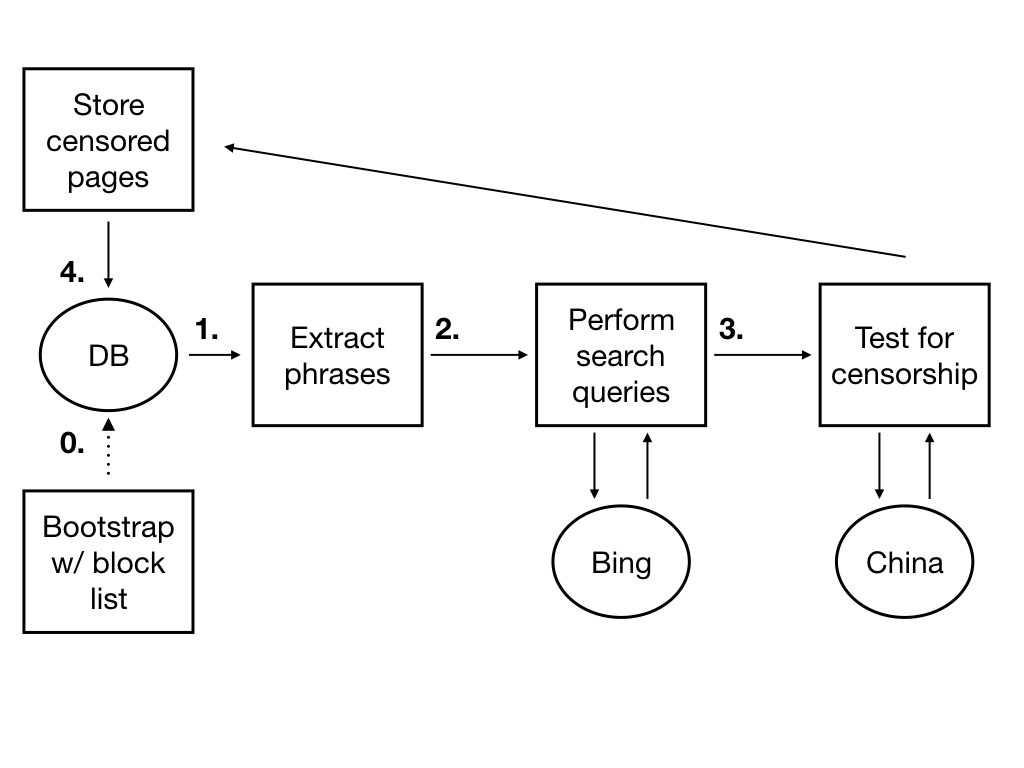
\includegraphics[scale=0.23]{figures/arch-2}
  \caption{\label{arch}CensorSeeker approach.}
\end{figure}

Figure~\ref{arch} summarizes CensorSeeker's approach to finding censored
websites. For the most part, CensorSeeker is similar to
FilteredWeb~\cite{darer2017filteredweb}. We start by bootstrapping a list of
webpages that are known to be censored, such as the Citizen Lab block
list~\cite{citizenlab:block}.
Then, we extract Chinese and English phrases that characterize these webpages.
Then, we use these phrases as search queries to find related webpages that
might also be censored. Finally, we test each search result for DNS
manipulation in China and feed the censored webpages back to the beginning of
the system. The rest of this section details the new capabilities of
CensorSeeker beyond the state of the art.

\subsection{Extracting multi-word phrases}
An n-gram is a building block for natural-language processing that
represents a sequence of ``n'' units of text, e.g. words. For example,
if we were to compute all of the bigrams of words in the English phrase
[\texttt{Chinese human rights violation}], we'd get \texttt{Chinese
human}, \texttt{human rights}, and \texttt{rights violation}. Similarly,
if we were to compute all the trigrams of words, we'd get
\texttt{Chinese human rights} and \texttt{human rights violation}. On the
other hand, if we simply extract unigrams from the sentence,
we'd be left with \texttt{Chinese}, \texttt{human}, \texttt{rights}, and
\texttt{violation}. As such, we believe that by combining unigrams
into bigrams and trigrams, we're able to learn more about the subject
of a webpage.

Unfortunately, computing the n-grams of words in Chinese text is
difficult because it is typically written without spaces, and there is
no clear indication of where characters should be separated. Computing
such boundaries in natural-language processing tasks is often
probabilistic, and depending on where characters are separated, one
can arrive at very different meanings for a given
phrase~\cite{stanford:segmenter}. For example, consider the
text \begin{CJK*}{UTF8}{gbsn}天花\end{CJK*}. This is considered a
Chinese unigram that translates to
``smallpox'' in English, but the character \begin{CJK*}{UTF8}{gbsn}
天\end{CJK*} on its own translates to ``sky'', and the
character \begin{CJK*}{UTF8}{gbsn}花\end{CJK*} on its own translates
to ``flower''. Given that we do not have domain-specific knowledge of
the webpages that we're analyzing, we consider a unigram to be
whatever the segmenter software in the Stanford CoreNLP library considers to be
a unigram, even if a Chinese unigram translates to multiple words in
English~\cite{tseng2005conditional, chang2008optimizing}.

We believe that using Chinese bigrams and trigrams for search queries
instead of individual English words is more effective for discovering
censored websites in China. For example, we know that websites that
express collective dissent are considered sensitive by the Chinese
government~\cite{king2013censorship}. If we used the words
\texttt{destroy}, \texttt{the}, \texttt{Communist}, or \texttt{Party}
individually as search terms, we might not get websites that express
collective dissent because the words have been taken out of
context. On the other hand, the phrase [\texttt{destroy the Communist
Party}] as a whole expresses collective dissent, which might enable us
to find many censored domains when used as a search term. We evaluate
the effectiveness of such phrases in Section \ref{phrases-eval}.

\subsection{Ranking phrases} \label{tf-idf}
To ``rank'' the phrases on a censored webpage, we use
term-frequency/inverse document-frequency (TF-IDF). TF-IDF is a
natural language technique that allows us to determine which phrases
best characterize a given webpage~\cite{ramos2003using}. It can be thought to work in three
steps. First, we compute the term-frequency for each phrase on a
webpage, which means that we count the frequency of each bigram and
trigram. Then, we compute the document-frequency for each phrase on a
webpage, which entails searching a Chinese corpus for the frequency of
a given phrase across all documents in the
corpus~\cite{phrasefinder}. Finally, we multiply the term frequency by
the inverse of the document frequency. The resulting score gives us an
idea of how important a given Chinese phrase is to a webpage.

Using this method, phrases like \begin{CJK*}{UTF8}{gbsn}1989年民主运
动\end{CJK*} [\texttt{1989 democracy movement}]
and \begin{CJK*}{UTF8}{gbsn}天安门广场示威\end{CJK*}
[\texttt{Tienanmen Square Demonstrations}] might rank highly on a
website about Chinese political protests. We would then use these phrases
as search terms in order to find related websites that might also be
censored. If we find a lot of censored URLs as a result, then we can
infer that the topic covered by that phrase is considered sensitive in China.

\subsection{Parsing Chinese text}
Before we can compute TF-IDF for a given webpage, we need to tokenize the
text. Doing so is simple enough for English because each word is separated by a
space. For languages such as Chinese, however, all of the words in a sentence are
concatenated, without any spaces between them. As such, we need to apply
natural-language processing techniques to perform fine-grained analysis
of the text on a webpage.

To do so, we make use of Stanford CoreNLP, a set of natural language
processing tools that operate on text for English, Arabic, Chinese, French,
German, and Spanish~\cite{corenlp2016suite}. For Chinese webpages, it allows us
split a sentence into a sequence of unigrams, each of which may represent
one word or even multiple words. By combining neighboring unigrams, then, we
can extract key phrases from a webpage that describe its content.

As previously mentioned, although FilteredWeb is concerned with finding webpages
that are censored in China, it is only able to parse text for the ISO basic
Latin alphabet~\cite{darer2017filteredweb}. By being able to parse Chinese text as
well as ISO Latin text, then, we are able to cover many more webpages and
extract regional information that may explain why a given webpage is
censored. In future work, we could make use of more intricate tools
from Stanford CoreNLP likes its part-of-speech tagger to identify
phrases that convey relevant information.

\begin{table}[b]
  \begin{center}
    \scalebox{0.80}{
    \begin{tabular}{ | l | r | r | r | }
      \hline
      Phrase length & Domains & Domains w/o Alexa Top 1000 \\ \hline
      Unigrams      & 1029    & 765 \\
      Bigrams       & 970     & 655 \\
      Trigrams      & 975     & 629 \\
      Total         & 1756    & \textbf{1125} \\
      \hline
    \end{tabular}}
  \end{center}
\caption{\label{breakdown} Total number of censored domains discovered.}
\end{table}

\begin{figure*}[t]
  \centering
  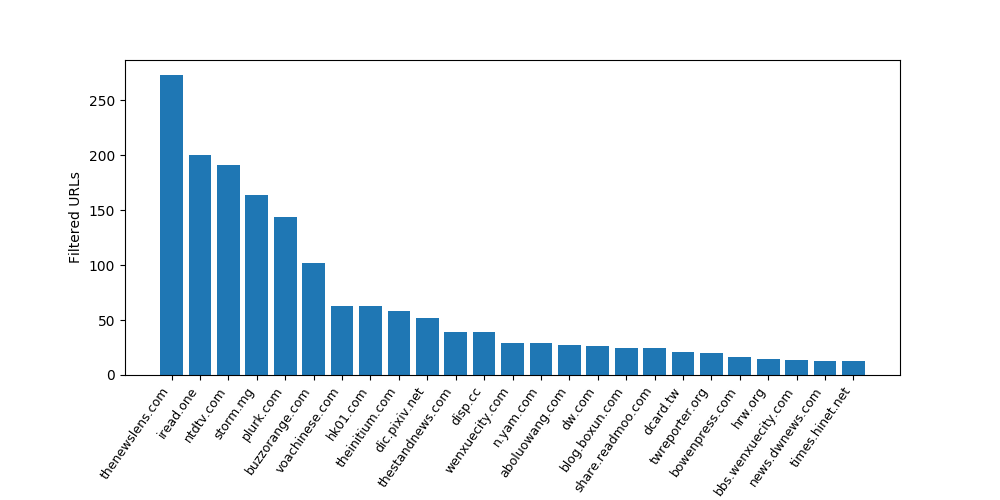
\includegraphics[scale=0.6]{figures/top-domains}
  \caption{\label{top-domains}Top censored domains by URL count.}
\end{figure*}

\section{Evaluation}

We performed a large-scale evaluation of our approach to
discover region-specific websites that are censored in China.  We
began by seeding with the Citizen Lab block list, which is
the most widely used list by censorship researchers. The list contains
220 webpages that either are blocked or have been alleged to be blocked in
the past. Since we only extract phrases from webpages that are
currently censored, we began by testing each webpage on the block list for
censorship. This left us with 108 unique webpages and 85 domains.

From November 11th, 2017 to January 9th, 2018, we used Bing's Search
API to search for websites related to known censored
websites~\cite{microsoft:bing}. According to the API, each call can
return at most 50 search results. Since it would be expensive to
perform multiple API calls for each search term, we limited ourselves
to one API call, i.e. 50 search results, per search term. For 
each website in the search results, we tested for censorship by
sending a DNS request to a set of controlled IP addresses in China
that don't belong to DNS servers. As with FilteredWeb, if we
received a DNS response, we inferred that the DNS request was
intercepted, and thus the tested website is
censored~\cite{darer2017filteredweb}. Finally, we performed three
separate evaluations to measure the effectiveness of different phrase
sizes for finding censored websites. With each evaluation, we only
extracted unigrams, bigrams, and trigrams, respectively. We also limited
each evaluation to 1,000,000 URLs to be consistent with the
methodology of FilteredWeb.

We also configured the Bing API calls so that any URLs from Blogspot,
Facebook, Twitter, YouTube, and Tumblr would be ignored. We did this
for a couple of reasons. For one, these websites are widely known to
be censored in China, so we would not be providing new information by
having these websites or their subdomains in our result
set. Furthermore, Tumblr and Blogspot assign a unique subdomain to
each user's blog, and in some cases we'd get a dozen blogs from a
single search query. In order to find culture-specific websites that
are normally buried by the top 50 search results, then, we need to
omit these blogs.
\begin{figure*}[t]
  \centering
  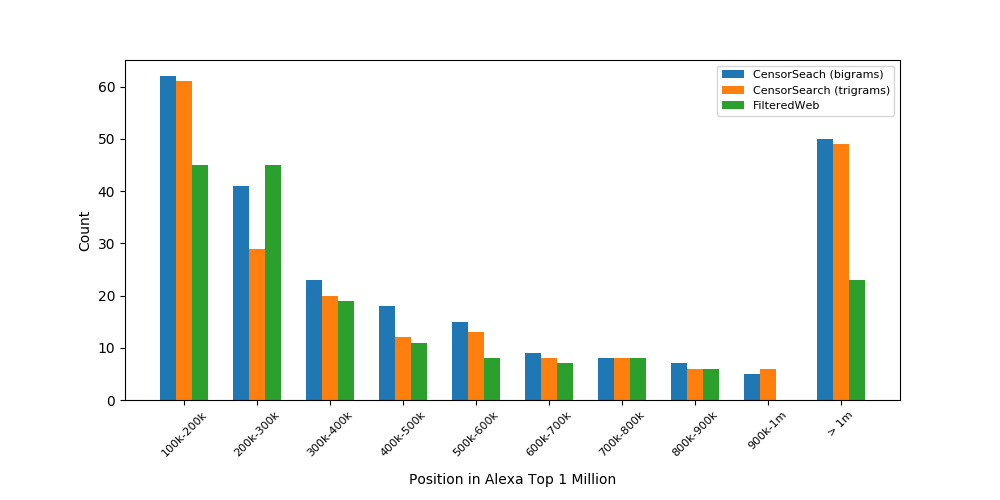
\includegraphics[scale=0.6]{figures/alexa}
  \caption{\label{alexa}Ranking of censored websites on Alexa Top 1 Million.}
\end{figure*}

\section{Results}
We reached several key insights from performing our
evaluations. First, we were able to discover hundreds of
censored websites that are not present on existing block
lists. Furthermore, we noticed that many websites on our block list
receive very little traffic. Lastly, we found that by using
politically-charged phrases as search terms, we were able to find a
disproportionately large amount of censored websites. The rest of this
section discusses the main findings in depth.

\subsection{Existing blocklists are incomplete}
\textit{By using natural-language processing on Chinese web pages, we
were able to discover hundreds of censored websites that are not
present on the Citizen Lab block list--the standard for censorship
measurements--and FilteredWeb's block list~\cite{darer2017filteredweb,
citizenlab:block}}. Furthermore, the set of websites that appeared the
most in our search results is almost entirely different from that of
FilteredWeb. Figure~\ref{top-domains} breaks down this result when
using unigrams, bigrams, and trigrams as search queries. These websites seem
to mainly cover Chinese human rights issues, news, censorship
circumvention, and more.

For instance, \texttt{wiki.zhtube.com} appears to be a Chinese
Wikipedia mirror. The web page for \texttt{zhtube.com} seems to be the
default page for a Chinese LNMP (Linux, NginX MySQL, PhP) installation
on a virtual private server~\cite{lnmp}. We found over 3000 URLs in
our dataset that point to this website, which suggests that many
Chinese websites are trying to circumvent the on-and-off censorship of
Wikipedia in China~\cite{wikipedia-china}. Furthermore,
\texttt{blog.boxun.com} is a United States-based outlet for Chinese
news that relies heavily on anonymous submissions. The owners of the
website note that ``Boxun often reports news that authorities do not
tell the public, such as outbreaks of diseases, human rights
violations, corruption scandals and disasters''~\cite{boxun-about}. As
such, the censorship of these websites might reflect the Chinese
government's policy of information control.

Furthermore, only three of the top 25 domains that we discovered are in
the top 50 domain list produced by FilteredWeb. Four of the top five
domains that we discovered--\texttt{ntdtv.com},
\texttt{storm.mg}, \texttt{cn.shafaqna.com}, and
\texttt{thenewslens.com}--are non-Western media websites that cover
Chinese news. \textit{Thus, by building on the
approach of FilteredWeb, we were able to produce a qualitatively
different block list}. We recommend putting these two block lists
together to create a single block list that is both wide in scope and
large in size.

Intuitively, we were able to find hundreds of qualitatively
different censored domains than those found by FilteredWeb because
we could extract Chinese-specific topics from web pages. We were able
to do so by using TF-IDF with a Chinese corpus to rank the
``uniqueness'' of Chinese phrases that appeared on a given
web page. For example, the trigram
\begin{CJK*}{UTF8}{gbsn}仅 限于 书面\end{CJK*} (``only written'') was poorly ranked on
\texttt{tianenmenmother.org}--a Chinese democratic activist group--
because although it appears frequently, it's a common phrase in
Chinese, according to the Chinese corpus on
PhraseFinder~\cite{phrasefinder}. On the other hand, the
trigram \begin{CJK*}{UTF8}{gbsn}自由 亚洲 电台\end{CJK*} (``Radio Free
Asia'') was highly ranked because it didn't appear frequently, and
it's an uncommon phrase in Chinese. It should also be noted that Radio
Free Asia is a broadcasting corporation whose stated mission is to
``provide accurate and timely news and information to Asian countries
whose governments prohibit access to a free
press''~\cite{rfa:about}. Thus, by scoring Chinese phrases with TF-IDF
against a Chinese corpus, we were able to determine which phrases are
``content-rich'' on a given web page.

\begin{table}[b]
  \begin{center}
    \scalebox{0.80}{
    \begin{tabular}{ | l | r | r | r | }
      \hline
      Phrase length & Domains & Domains w/o Alexa Top 1000 \\ \hline
      Unigrams      & 1029    & 765 \\
      Bigrams       & 970     & 655 \\
      Trigrams      & 975     & 629 \\
      Total         & 1756    & \textbf{1125} \\
      \hline
    \end{tabular}}
  \end{center}
\caption{\label{breakdown} Total number of censored domains discovered.}
\end{table}

\subsection{China blocks many unpopular websites}
Figure~\ref{alexa} shows the ranking of the websites we discovered on
the Alexa Top 1,000,000. Notably, many of the websites we discovered
are spread throughout the tail of the list, and some of the websites
are not even on the list at all. \textit{Given that the top 100,000 websites
likely receive the vast majority of traffic on the Internet, we can
infer that censors in China are not just interested in blocking
``big-name'', popular websites.} They are actively seeking out websites
of \textit{any size} that contain ``sensitive'' content. We also
discovered a number of websites that fall outside the Alexa Top
1,000,000 altogether. Without the use of an automated system that can
discover censored websites, it's unlikely that the public would even
be aware that these websites are blocked.

Furthermore, we were able to consistently discover \textit{more} unpopular
censored domains with our approach than FilteredWeb. For domains that
rank between 200,000 and 300,000 on the Alexa Top 1,000,000,
FilteredWeb was able to discover more domains, but in every other bin of
100,000 ranks we discovered more. Notably, between the ranks of 900,000
and 1,000,000, FilteredWeb did not discover \textit{any} censored domains, and
we discovered far more domains that fall outside of the Alexa Top
1,000,000 altogether. This suggests that the use of Chinese phrases
as search queries allowed us to uncover a significant number of
websites that would otherwise be unknown to censorship researchers.

\begin{figure}[t]
  \centering
  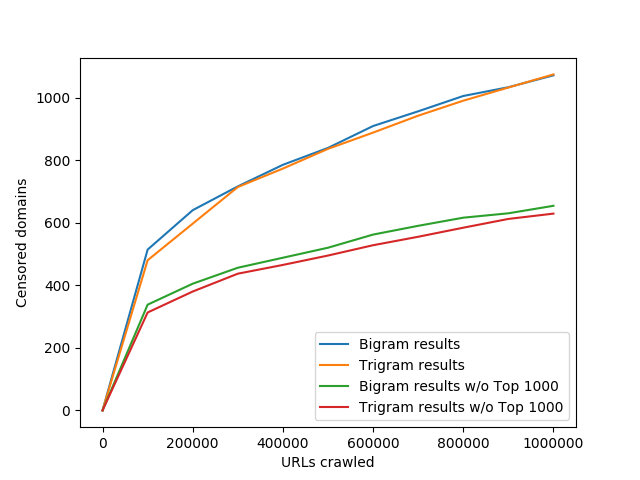
\includegraphics[scale=0.5]{figures/urls-crawled}
  \caption{\label{censored-vs-urls} Censored domains discovered over unique URLs crawled. }
\end{figure}

\begin{table}[b]
  \begin{center}
    \scalebox{0.9}{
      \begin{tabular}{ l | l | c }
        Chinese & English & Censored domains \\ \hline
        \begin{CJK*}{UTF8}{gbsn}王歧山\end{CJK*} & Wang Qishan & 74\% \\
        \begin{CJK*}{UTF8}{gbsn}李洪志\end{CJK*} & Li Hongzhi & 64\% \\
        \begin{CJK*}{UTF8}{gbsn}郭伯雄\end{CJK*} & Guo Boxiong & 62\% \\
        \begin{CJK*}{UTF8}{gbsn}胡锦涛\end{CJK*} & Hu Jintao & 56\% \\
        \begin{CJK*}{UTF8}{gbsn}胡平\end{CJK*}  & Hu Ping & 54\% \\
        \begin{CJK*}{UTF8}{gbsn}Morty\end{CJK*} & Morty & 52\% \\
        \begin{CJK*}{UTF8}{gbsn}命案\end{CJK*}  & Homicide & 52\% \\
        \begin{CJK*}{UTF8}{gbsn}特首\end{CJK*}  & Chief executive & 52\% \\
        \begin{CJK*}{UTF8}{gbsn}Vimeo\end{CJK*} & Vimeo & 50\% \\
        \begin{CJK*}{UTF8}{gbsn}中情局\end{CJK*} & CIA & 50\% \\
      \end{tabular}}
  \end{center}
  \caption{\label{effective-unigrams}Sample of unigrams with
    significant blockrates}
\end{table}

Table \ref{breakdown} shows the breakdown of how many censored
websites we discovered. By using unigrams, we were able to discover
765 domains that are not on any publicly available block list. By
using bigrams, we were able to discover 655 censored domains. Lastly,
by using trigrams, we were able to discover 629 censored domains. In
total, we discovered 1125 censored domains, none of which are on the
Alexa Top 1000~\cite{alexa:top1000}. Each of these evaluations were
performed with 1,000,000 unique URLs, consistent with the methodology
of FilteredWeb~\cite{darer2017filteredweb}. Figure
\ref{censored-vs-urls} shows how many censored domains we discovered
as a function of unique URLs crawled for each evaluation.

\begin{table*}[t]
  \begin{center}
    \scalebox{0.9}{
      \begin{tabular}{ l | l | c }
        Chinese & English & Censored domains \\ \hline
        \begin{CJK*}{UTF8}{gbsn}中共\end{CJK*} \begin{CJK*}{UTF8}{gbsn}威胁\end{CJK*} & Chinese Communists threaten & 50\% \\
        \begin{CJK*}{UTF8}{gbsn}声明的\end{CJK*} \begin{CJK*}{UTF8}{gbsn}反共产主义\end{CJK*} & Declared anti-communist & 44\% \\
        \begin{CJK*}{UTF8}{gbsn}中国共\end{CJK*} \begin{CJK*}{UTF8}{gbsn}产党的公共安全\end{CJK*} & Public security of the CPC & 42\% \\
        \begin{CJK*}{UTF8}{gbsn}北京\end{CJK*} \begin{CJK*}{UTF8}{gbsn}清洁\end{CJK*} & Beijing clean-up & 40\% \\
        \begin{CJK*}{UTF8}{gbsn}江泽民\end{CJK*} \begin{CJK*}{UTF8}{gbsn}胡锦涛\end{CJK*} & Jiang Zemin Hu Jintao & 40\% \\
        \begin{CJK*}{UTF8}{gbsn}迫害\end{CJK*} \begin{CJK*}{UTF8}{gbsn}活动\end{CJK*} & Persecution
                                                     activities & 40\% \\
        \begin{CJK*}{UTF8}{gbsn}官员\end{CJK*} \begin{CJK*}{UTF8}{gbsn}呼吁\end{CJK*} & Officials called on & 36\% \\
        \begin{CJK*}{UTF8}{gbsn}重的\end{CJK*} \begin{CJK*}{UTF8}{gbsn}公民\end{CJK*} & Heavy Citizen & 36\% \\
        \begin{CJK*}{UTF8}{gbsn}非法\end{CJK*} \begin{CJK*}{UTF8}{gbsn}拘留\end{CJK*} & Illegal detention
                          & 36\% \\
        \begin{CJK*}{UTF8}{gbsn}不同\end{CJK*} \begin{CJK*}{UTF8}{gbsn}的民主\end{CJK*} & Different Democratic & 34\% \\
      \end{tabular}}
  \end{center}
  \caption{\label{effective-bigrams}Sample of bigrams with significant
    block rates}
\end{table*}

\begin{table*}[t]
  \begin{center}
    \scalebox{0.9}{
      \begin{tabular}{ l | l | c }
        Chinese & English & Censored domains \\ \hline
        \begin{CJK*}{UTF8}{gbsn}北戴\end{CJK*} \begin{CJK*}{UTF8}{gbsn}河\end{CJK*} \begin{CJK*}{UTF8}{gbsn}会议\end{CJK*} & BEIDAIHE meeting & 54\% \\
        \begin{CJK*}{UTF8}{gbsn}中国\end{CJK*} \begin{CJK*}{UTF8}{gbsn}共产党\end{CJK*} \begin{CJK*}{UTF8}{gbsn}的宗教政策\end{CJK*} & The Chinese Communist Party's religious policy & 42\% \\
        \begin{CJK*}{UTF8}{gbsn}采取\end{CJK*} \begin{CJK*}{UTF8}{gbsn}暴力\end{CJK*} \begin{CJK*}{UTF8}{gbsn}镇压\end{CJK*} & To take a violent crackdown & 38\% \\
        \begin{CJK*}{UTF8}{gbsn}香港\end{CJK*} \begin{CJK*}{UTF8}{gbsn}政\end{CJK*} \begin{CJK*}{UTF8}{gbsn}治\end{CJK*} & Hong Kong Politics & 34\% \\
        \begin{CJK*}{UTF8}{gbsn}欧洲\end{CJK*} \begin{CJK*}{UTF8}{gbsn}议会\end{CJK*} \begin{CJK*}{UTF8}{gbsn}决议\end{CJK*} & European Parliament Resolution & 32\% \\
        \begin{CJK*}{UTF8}{gbsn}新\end{CJK*} \begin{CJK*}{UTF8}{gbsn}唐\end{CJK*} \begin{CJK*}{UTF8}{gbsn}王朝\end{CJK*} & New Tang Dynasty & 32\% \\
        \begin{CJK*}{UTF8}{gbsn}恐怖\end{CJK*} \begin{CJK*}{UTF8}{gbsn}事件\end{CJK*} \begin{CJK*}{UTF8}{gbsn}。\end{CJK*} & A terrorist event. & 32\% \\
        \begin{CJK*}{UTF8}{gbsn}天安\end{CJK*} \begin{CJK*}{UTF8}{gbsn}门广\end{CJK*} \begin{CJK*}{UTF8}{gbsn}场示威\end{CJK*} & Tienanmen Square Demonstrations & 32\% \\
        \begin{CJK*}{UTF8}{gbsn}敦促\end{CJK*} \begin{CJK*}{UTF8}{gbsn}美国\end{CJK*} \begin{CJK*}{UTF8}{gbsn}政府\end{CJK*} & Urging the US government & 32\% \\
        \begin{CJK*}{UTF8}{gbsn}1989\end{CJK*} \begin{CJK*}{UTF8}{gbsn}民主\end{CJK*} \begin{CJK*}{UTF8}{gbsn}运动\end{CJK*} & 1989 democracy movement & 30\% \\
      \end{tabular}}
  \end{center}
  \caption{\label{effective-trigrams}Sample of trigrams with
    significant blockrates}
\end{table*}

\subsection{Political phrases are highly effective}
\label{phrases-eval}

We also wanted to see if there is a correlation between the
presence of certain phrases and whether or not a given website is
censored, even if we have no ground truth.  For example, if we make a search
for \begin{CJK*}{UTF8}{gbsn}中国侵犯人权\end{CJK*} (Chinese human
rights violation) and find that a particular search result is
censored, then we cannot be certain whether the presence of that phrase
\textit{caused} the website to be blocked. Even if we assume 
that a censor is manually combing through search engines to find
sensitive websites, the website could have been blocked because it
contained totally different content.

Nevertheless, there seems to be some correlation for certain
phrases. Table~\ref{effective-unigrams} shows a sample of unigrams
that returned the most number of unique filtered domains from
Bing. For example, the top four unigrams--Wang Qishan, Li Hongzhi, Guo
Boxiong, and Hu Jintao--are the names of controversial figures in
Chinese history. Li Hongzhi is the leader of the Falun Gong spiritual
movement, whose practitioners have been subject to persecution and
censorship by the Chinese government since
1999~\cite{freedomhouse:falun}. Similarly, Guo Boxiong is a former top
official of the Chinese military that was sentenced to life in
prison in 2016 for accepting bribes, according to the Chinese
government~\cite{guardian:guo}. Thus, if a Chinese website discusses
these people, the website may become censored for containing
``sensitive'' content.

There are also bigrams that correlate with a large percentage of
censored domains, but they are more explicitly political than the
unigrams. Table~\ref{effective-bigrams} shows this result. First, most
of the bigrams refer to the Chinese Communist Party in some
way. Phrases such as \begin{CJK*}{UTF8}{gbsn}中共的威胁\end{CJK*}
(Chinese Communists threaten), \begin{CJK*}{UTF8}{gbsn}江泽民胡锦
涛\end{CJK*} (Jiang Zemin Hu Jintao), and \begin{CJK*}{UTF8}{gbsn}中国
共产党的治安\end{CJK*} (Public security of the CPC) do not necessarily
convey sensitive information, but they nonetheless refer to the
government of China. On the other hand, some phrases clearly refer to
political dissent, such as \begin{CJK*}{UTF8}{gbsn}官员呼吁\end{CJK*}
(Officials called on), \begin{CJK*}{UTF8}{gbsn}迫害活动\end{CJK*}
(Persecution activities), \begin{CJK*}{UTF8}{gbsn}非法拘留\end{CJK*}
(Illegal detention), and \begin{CJK*}{UTF8}{gbsn}宣称反共\end{CJK*}
(Declared anti-communist).

We see a similar result with trigrams, as shown by
Table~\ref{effective-trigrams}. Phrases that stand out
include \begin{CJK*}{UTF8}{gbsn}中国共产党的宗教政策\end{CJK*} (The
Chinese Communist Party's religious policy), \begin{CJK*}{UTF8}{gbsn}
天安门广场示威\end{CJK*} (Tienanmen Square
demonstrations), \begin{CJK*}{UTF8}{gbsn}1989年民主运动\end{CJK*}
(1989 democracy movement), and \begin{CJK*}{UTF8}{gbsn}采取暴力镇
压\end{CJK*} (To take a violent crackdown). Interestingly, we also see
that discussion of China's religious policy, the ``New Tang
Dynasty''--a religious radio broadcast located in the United States--,
and European Union legislation may also be considered sensitive
content.~\cite{china-religion}. \textit{Together, these results
suggest that references to collective political dissent are highly
likely to be censored}. This is consistent with the findings of King
et al.~\cite{king2013censorship}.


% \section{Discussion}
% There are several possible explanations for why CensorSeeker didn't find
% more censored domains than FilteredWeb. Our use of phrases as search
% terms tended to return websites that cover particular issues, and
% these websites may not as heavily censored by the Chinese
% government. This could mean that either a) the censors just aren't
% aware of many of the non-censored domains we found, or b) the censors
% are more concerned about major media outlets and Western
% websites. However, we can't be sure of either of these hypotheses
% without insider knowledge of how websites are chosen to be censored in
% China.

% Nonetheless, we could combine our results with Darer's results
% to create the largest publicly-available block list for China. Such a
% contribution would be valuable to researchers that are interested in
% understanding socio-political trends that drive censorship in China.

% \section{Limitations}
% A significant limitation of our work is our method for extracting significant
% terms and phrases from webpages. As previously discussed, we use TF-IDF to
% determine which terms are most signicicant on a given webpage. We ignore
% stopwords that don't provide significant information on their own, e.g. ``and'',
% ``of'', and ``the''. However, our algorithm still extracted a siginificant
% number of Chinese tags that were not very useful, such as dates and times. We believe
% this occurs on websites that have a significant amount of text that can't be
% found in the corpus. In such a case, the algorithm is foced to choose less
% significant that can be found in the corpus. One way to get around this is to
% find a larger corpus for Chinese text, but to our knowledge, the Google N-grams
% corpus is the largest publicly-available corpus.

% Another limitation of CensorSeeker is its reliance on the top 50 search
% results returned by Bing from each search. For many searches, popular
% websites like Wikipedia, Yahoo, and Wenxuecity appeared over and over
% again in the search results. Although the phrases that we extracted
% from these websites were helpful in discovering more censored
% websites, these three domains in particular dominated our search
% results. As such, we may have discovered more censored websites by
% skipping over the top 50 search results. This would be an interesting
% direction for future work.

% Lastly, CensorSeeker only tests if URLs are blocked at the domain level. We do not
% test to see if individual URLs under a given domain are blocked through IP
% filtering or deep-packet inspection. While our results are interesting on their
% own in that we discovered a significant amount of censored domains, we may be
% missing URLs that are not blocked at the domain level but are nonetheless
% censored through other methods. If we were able to perform such a fine-grained
% analysis, we would have a more precise understanding of what content is
% considered sensitive in China.


% \section{Future work}
% It would be interesting to test each censored domain on real resolvers located
% in China to determine whether or not they are only censored in certain
% regions. Previous work has shown that censorship in China seems to differ among
% regions, suggesting that it may be a rather decentralized operation among
% ISPs~\cite{pearce:global}. For example, the Chinese government might tell ISPs
% to filter out certain \textit{categories} of websites, e.g. Tibetan news, but
% they also might leave it up to the ISPs to determine amongst themselves which
% \textit{websites} should be censored. As such, it would be interesting to identify
% resolvers in different regions in China and test our set of censored domains
% against each resolver.

% Furthermore, we could incorporate Iris into CensorSeeker to account for different
% forms of manipulation. Our method of evaluation follows that of FilteredWeb
% in that we query domains against Chinese IPs that do not actually belong to
% resolvers. If we get actually get a response back from the IP, then we know that
% our query was poisoned along the way. However, there may be more subtle forms of
% manipulation happening once our request reaches China. For example, we could
% look at the time-to-live information from each DNS response to infer
% if requests are going through the same middleboxes.

% We could also repeat this experiment to measure censorship in
% Russia. This may prove challenging given that we don't have a
% tokenizer for Russian phrases. Nonetheless, we think that we could
% still get good results by naiively tokenizing Russian text around
% spaces and punctuation. Our goal would be to to show that CensorSeeker
% performs in different countries and different languages.

% Lastly, we could reach out to the maintainers of censorship
% measurement platforms like OONI and ICLab to continously test these
% domains over time. Some websites may become uncensored over time, and
% it would be interesting to have a number of volunteers that could
% measure such a phenomenon against our dataset. This may prove
% challenging given that platforms like OONI require websites that are
% tested to be vetted as legitimate and non-malicious; we have a lot of
% domains that would need to be manually vetted. Nonetheless, if this
% could be done, we could have a more complete understanding of how
% censorship changes over time.

\balance
\section{Conclusion}
We built a block list of 757 censored websites in China that are not
present on the largest block
list~\cite{darer2017filteredweb}. Furthermore, our list is 8.5$\times$
larger than the most widely used block
list~\cite{citizenlab:block}. It contains human rights organizations,
minority news outlets, religious blogs, political dissent groups,
privacy-enhancing technology providers, and more. We've open-sourced
our source code and block list on GitHub with the GPL
license~\cite{censorsearch-lists}.

Automatically detecting which websites are censored in a given country is an
open problem. Approaches like ours and that of FilteredWeb are steps in the
right direction, but there is more work to be done.  One way of improving
our work would be to experiment with advanced natural-language processing
techniques to identify better search terms. For example, we could try using
Stanford CoreNLP's part-of-speech tagger to identify phrases that describe
some action against the Chinese government. This approach might
identify the following phrase: ``Chinese citizens protest against the Communist Party on June
4th''. We believe that using such culture-specific phrases as search terms
would enable us to discover even more websites that are censored in China.

% We could also try running CensorSeeker against different search engines to see
% if we get different result sets. It might be the case that one search engine
% is able to find more censored websites than the others. It might also be the
% case that one search engine is better at finding culture-specific websites
% than the others. To our knowledge, Bing is the only search engine that
% provides a public API, so we would have to coordinate with other search
% engines to make this happen.


\section*{Acknowledgements}
We thank the anonymous FOCI '18 reviewers for their helpful
feedback. We also thank Chris Miller for help with setting up a 
machine that was used for data analysis. This work was supported by
[...] and [...].

\newpage

{\footnotesize
 \bibliographystyle{acm}
 \balance\bibliography{../common/bibliography}}


\end{document}
